
%
\RequirePackage{fix-cm}
%
\documentclass[table,smallextended]{svjour3}       % onecolumn (second format)
\usepackage{kotex}                           % https://crmn.tistory.com/34

\smartqed  % flush right qed marks, e.g. at end of proof
%
\usepackage{graphicx}
\usepackage{algorithm}
\usepackage{arevmath}     % For math symbols
\usepackage[noend]{algpseudocode}
\usepackage[margin=1.5in]{geometry}    % For margin alignment


%TABLE
\usepackage{PTSansNarrow}
\usepackage[T1]{fontenc}
\usepackage{array,tabularx}
\usepackage[most]{tcolorbox}


\begin{document}

\title{비잔틴 장애 허용 상태 복제 알고리즘 조사 및 분석을 통한 분산 프로그래밍 언어 설계 가능성 조사}
% \subtitle{Do you have a subtitle?\\ If so, write it here}

%\titlerunning{Short form of title}        % if too long for running head

\author{최창원         \and
        조은선 %etc.
}

%\authorrunning{Short form of author list} % if too long for running head

\institute{최창원 \at
              충남대학교 PLAS LAB,
              \email{qwefgh90@naver.com}           %  \\
%             \emph{Present address:} of F. Author  %  if needed
           \and
              조은선 \at
              충남대학교 PLAS LAB,
              \email{eschough@cnu.ac.kr}
}

\date{작성일: 2020/12/08}
% The correct dates will be entered by the editor


\maketitle

\renewcommand{\abstractname}{초록}
\renewcommand{\refname}{참조}
\begin{abstract}
현재 연구주제로 고려하고 있는 것은 분산 시스템 개발용 언어 개발이다. 이러한 분산 시스템을 위한 언어를 개발한다는 것은
분산 시스템을 설계하는 것과 유사하다고 생각한다. 예를들어 한 노드에서 다른 노드의 메서드를 원격 호출한 경우 
양쪽의 상태를 동시에 갱신해야할 수도 있고 같은 네트워크에 참여 중인 노드의 상태를 변경해야하는 경우도 있을 것이다.
이렇게 각 노드, 프로세스, 컴포넌트가 어떻게 서로 통신을 하고 상태를 동기화 하는지 연구를 할 필요가 있다.
본 서베이 논문은 비잔틴 장애를 허용(Byzantine-fault-tolerant)하는 
상태 머신 복제(State Machine Replication) 알고리즘과 블록체인의 분산 원장에 활용되는 기술 등을 다룬다. 
현대의 대부분의 서비스는 분산된 노드가 서로 정보를 주고 받으며 동작한다.
이 과정에서 분산된 노드간에 동일한 설정 유지할때나 하나의 상태를 갖는 분산 컴포넌트를 개발할때
상태 머신 복제 알고리즘은 중요한 역할을 하게 된다. 상태 복제 알고리즘은 오랫동안 연구되어 왔으며 최근 블록체인의
발전으로 그 중요성이 부각되고 있다. 또한 HotStuff 같은 알고리즘의 등장으로 성능이 획기적으로
개선되기도 하였다. 이 서베이 논문은 비잔틴 장애 허용 알고리즘을 다루고
알고리즘 간에 성능 및 장단점을 비교하여 설명한다.

\end{abstract}

\section{서론}
\label{intro}
소프트웨어의 재활용성 덕분에 
아이디어만 있다면 새로운 앱을 구현하는데 많은 시간을 들이지 않을 수 있다.
언어와 개발 도구의 발달, 오픈소스와 생태계의 발전, 웹 기술의 발전은 
재활용 가능한 소프트웨어를 누구나 쉽게 소비하거나 또는 생산자로서 구현하고 배포할 수 있게 하였다.
단순한 라이브러리나 프레임워크 수준을 넘어선 API 서비스의 등장으로
코드 뿐만 아니라 서비스 자체를 재활용하는 것이 가능해졌다. 분산된 노드의
통신이 빈번한 환경에서는 악의적인 공격자에 의해 해킹을 당하기 쉽다.
해커는 시스템 중 약한 부위를 공격하여 루트권한을 획득하고 제어서버를 통해 
시스템을 원하는 대로 조작할 수 있다. 위와 같은 분산된 환경에서 해커의 공격을
대응하는 것이란 개발자 입장에서 단순히 시스템의 장애를 해결하는 것
이상의 어려운 일이다. 또한 점점 시스템에 많고 중요한 데이터가 저장되기 때문에 악의적인 공격을
당했을때 그 피해는 어마어마하다. 

다양한 분산 환경 중 여러 노드가 하나의 시스템 처럼
동일한 상태를 유지하고 서비스를 제공하는 경우가 있다.
특히 악의적인 노드가 존재하는 비잔틴 문제가 있더라도 시스템이
중요한 동작할 수 있게 해주는 비잔틴 장애 허용 상태 머신 복제 알고리즘은
보안성을 강화하기 위해 널리 활용되는 알고리즘이 되었다.
항상 시스템을 보호해주는 알고리즘은 아니고 \(3f+1\)개의 노드 중 f개 이하로 
결함있는 노드가 유지될때 문제없이 상태를 복제할 수 있게한다.

흔히 알려진 것 처럼 상태 머신 복제 시스템은 safety와 liveness 성질을 가지고 있어야 한다.
safety는 사용자가 전송한 시스템의 상태를 갱신하는 일련의
명령을 모든 노드가 동일한 순서대로 실행하여 같은 상태를 갖게해주는 능력이다.
liveness는 사용자 요청에 대한 응답을 해주는 능력을 의미한다.

동기적인(Synchronous)\cite{Synchron92}\cite{buchman2016tendermint} 모델은 결정된 제한 시간이 있어서 공격자가 결함없는 노드의 메시지를
그 시간 만큼만 지연시킬 수 있는 모델을 의미한다.
비동기적인(Asynchronous)\cite{Synchron92}\cite{buchman2016tendermint} 모델은 공격자가 제한할 수 있는 시간은 결정되어 있지 않으며
결함없는 노드가 보낸 메시지는 메시지는 결국 도달하는 모델을 의미한다.

부분 동기화(Partial synchrony)\cite{Synchron92}\cite{buchman2016tendermint} 모델은 일시적인 순간에만 비동기적 모델을 유지하고(공격 받는 상황) 
GST(Global Stabilization Time) 이후에는 동기적 속성을 유지하는 모델이다.
GST는 공격자가 이벤트를 발생시키는 예측할 수 없는 특정 시점이다.

\begin{itemize}
  \item GST는 알려지지 않은 유한한 시간이 지난 시점이다.
  \item t라는 시점에 전송된 모든 메시지는 \(max\{t,GST\}+\Delta\) 안에 도달한다.
\end{itemize}


최근에 상태 복제 머신이 활용되는 분야 중 하나는 블록체인(Blockchain)이
다. 블록체인은 동일한 기록을 갖는 분산원장으로 구성된다. 일반적으로 모든
분산 원장은 동일한 암호화페 거래내역을 저장해야 하며, 거래 요청 처리 순서를
동기화하여 처리해야 한다. 여기서 각 분산된 노드의 상태는 계좌내역(계좌번호,
잔액 등)이고, 이 상태를 모두 동일하게 복제하기 위해 상태 머신 복제 알고리즘이
사용된다.

예를들어 비트코인\cite{nakamoto2019bitcoin}은 작업증명(Proof of Work) 알고리즘과 Longest Chain
Rule을 활용하여 상태를 복제한다. 여러 복제본이 Proof of Work를 통해 블록 블록을
찾은 뒤 전파하여 동기화하고 Longest Chain Rule을 이용하여 포크 문제를 해결한다.
작업증명 알고리즘은 본래 서비스 거부 공격을 방어하기 위해 개발되었지만, 
비트코인에서 각 노드간 동일한 블록체인을 동기화할때 사용되면서 유명해졌다.

초기 버전 이더리움\cite{buterin2013ethereum} 같은 경우도 ethash를 적용한 작업증명 알고리즘과 고스트 프로토콜을
이용하여 상태 복제를 수행하고 및 포크 문제를 다루었다. 블록체인은 이처럼 초기에는 
서비스 거부 공격을 방어할 수 있는 작업증명 같은 보안성이 강한 알고리즘을 채택하였다.
이러한 시스템을 붕괴하기 위해서는 비잔틴 노드가 전체 노드의 51\% 이상이 되어야 하므로
해커들 입장에서도 해킹에 필요한 비용이 너무 비싸서 블록체인 자체를 공격하는 것은
어렵다고 한다.

하지만 블록체인 특성상 지리적으로 떨어진 노드가 많아서 포크 문제가 빈번하게 발생했고
Ghost 프로토콜 등을 이용해 이 문제를 다룰 수 있더라도, 한쪽 블록 전체를 버리게 됨으로써 
블록을 낭비하는 문제는 여전히 남아있었다. 그래서 이더리움 2.0에서는 지분증명과
같은 알고리즘을 지원하기 시작하였다.

블록체인 분야에서 사용되기도 하는 널리 알려진 PBFT(Practical Byzantine Fault Tolerance)는 
비동기 환경에서 비잔틴 문제를 해결할 수 있는
최초의 알고리즘이다. 순서 합의부터 결과 커밋까지 3가지 단계 Pre-Prepare, Prepare,
Commit로 구성되며 Pre-Prepare과 Prepare 단계는 동일한 순서로 명령이 실
행되는 것을 보장하며, Prepare과 Commit 단계는 커밋된 명령이 여러 뷰에서
완전히 정렬되는 것을 보장한다. 이후 PBFT의 성능을 개선한 많은 변형이 탄생
하였다. 현대에 쓰기에는 다소 성능이 느린 문제가 있다.

그리고 2019년 현대 시스템 환경에서 PBFT보다 빠르고 실용적인 리더 기반
상태 머신 복제 알고리즘 HotStuff\cite{yin2019hotstuff}가 등장하였다. 
HotStuff는 리더 기반 프로토콜로 부분적으로 동기 모델(Partially Synchronous Model)에서 동작하는 상태
머신 복제 알고리즘이다. 네트워크 커뮤니케이션이 동기적일때 네트워크 지연시
간의 속도에 맞춰 합의에 도달할 수 있게 해주는 responsiveness 속성을 보장한다.
그리고 복제본의 수에 선형적인 통신 복잡도를 갖게 해주며 합의 시간이 통신 지연시간 만큼 걸리는
linearity를 보장한다. 아마 HotStuff는 위 2가지 속성을 갖는 최초의 부분 동기화 BFT 복제 프로토콜이며,
거대한 복제 서비스에서 활용될 수 있는 여러가지 성능 최적화를 제공한다.

그리고 같은 해인 2019년에 LibraBFT라는 Libra 블록체인을 위한 알고리즘이 등장한다.
LibraBFT는 HotStuff 알고리즘을 기반으로 몇가지 아이디어가
추가된 알고리즘이다. LibraBFT는 새로운 라운드 동기화 매커니즘을 제공하며,
결함있는 리더 노드가 존재하더라도 제안이 커밋되는 것을 허용하는 nil-block
투표 방식 등을 제공한다.


\section{논문 분석}
\label{sec:1}
주로 블록체인(Blockchain)에서 활용되는 합의(Consensus) 알고리즘이나
널리 알려진 상태 머신 복제(State Machine Repliacation)을 요약하고
각 알고리즘의 특징과 장단점 등을 설명할 것이다. 그리고 상세한
프로토콜을 설명한다.

\subsection{Practical Byzantine Fault Tolerance}
정부나 산업에서 점점 정보시스템에 대한
의존성이 커지면서 악의적인 공격이 성공하였을때 그 피해가 점점 커지게 되었다.
그리고 시스템에 점점 많은 기능이 들어가고 복잡해지면서 소프트웨어 버그가 많아지게 되었다.
그래서 자의적인 행동을 하는 비잔틴 행동(Byzantine behavior)으로 부터 시스템을
보호하는 비잔틴 장애 허용 알고리즘의 중요성이 커지게 되었다.

PBFT(Pratical Byzantine Fault Tolerance)\cite{castro1999practical}는
1999년 Miguel Castro와 Barbara Liskov가 작성한 상태 머신 복제 알고리즘이다.
당시 이 논문이 발표되기전 소개되었던 알고리즘들은 동기적 환경에서 동작하거나
실제로 사용되기에는 너무 느렸다. 그래서 인터넷 환경과 같은 비동기 환경에서
비잔틴 문제를 허용하는 알고리즘이 필요하였고 PBFT가 등장하였다. 이 알고리즘은
결함있는 노드가 많아도 \([\frac{n-1}{3}]\)개 일때 safety와 liveness를 제공한다.

PBFT 이전에 등장한 알고리즘은 문제점을 크게 2가지 문제를 가지고 있었다. 
먼저 이론적으로 가능한지만 구현해서 사용하기에는 비효율적이고 어려웠다는 것이고
메시지 지연 시간과 처리 속도의 상한 값을 고정하는 동기화 가정(Synchrony Assumption)을 적용했다는 것이다.
Rampart나 SecureRing같은 알고리즘은 실용적이지만 정확성을 위해 동기화 가정에 의존하고 있었다.
동기화 가정은 악의적인 가정에 매우 취약하다. 공격자는 결함없는 노드를 그들 사이의 통신을 지연시키고
그 노드들이 결함있게 여겨지거나 복제 그룹에 의해 배제 당하게끔 하여 서비스의 안정성에 손상을 일으킬 수 있다.
PBFT는 동기화 가정에 의존하지 않기 때문에 저런 공격에 내성을 지니고 있다.

이 알고리즘은 상태 머신 복제 알고리즘이며 분산된 노드의 구성은 뷰(View)라는 단위로 관리된다.
뷰는 Primary와 여러개의 Backup으로 구성된다.
Primary는 사용자의 요청을 처리하기 위해 프로토콜을 시작하는 역할을 하는 복제본이다.
그리고 알고리즘의 동작을 위해 2가지 요구사항이 필요하다.
모든 복제본은 같은 순서의 요청 실행에 같은 상태를 갖도록 하기 위해
\textit{결정적(Deterministic)} 속성을 가져야하며 초기에 동일한 상태에서 시작해야 한다.

그리고 safety와 liveness 속성을 유지하기 위해 반드시 충족해야할 \(3f+1\)이라는 조건도 존재한다.
\(3f+1\)은 safety와 liveness를 위한 최소한의 복제본 숫자이다. 여기서 f는 결함있는 노드를 의미한다.
\(n\)개의 복제본이 있을때 f개의 응답하지 않는 결함있는 노드가 있을 수 있으며, f개의 결함이 있으나 응답하는 노드
f개의 결함이 있으나 응답하지 않는 노드가 있을 수 있다. 이때 메시지를 보내는 정상적인 노드의 개수는 결함을 가진
응답하는 노드의 개수보다 많아야 한다. 이는 수식으로 \(n-2f > f\) 즉, \(n >= 3f+1\)로 표현되고
이 조건이 만족되었을때 위의 2가지 속성이 보장되는 것이다.

primary가 사용자 요청 \textit{m} 받으면서 3단계 프로토콜을 시작한다.
3단계는 pre-prepare, prepare, commit이며 pre-prepare과 prepare 단계는
같은 뷰에 있는 여러개의 요청 순서를 정렬하기 위해 존재한다.
prepare, commit 단계는 모든 뷰를 거쳐 커밋된 요청들의 순서를 정렬하기 위해 존재한다.

먼저 pre-prepare 단계에서는 primary는 요청에 시퀀스 번호 \(n\)을 요청에 할당한다.
그리고 pre-prepare 메시지 \(((PRE-PREPARE,v,n,d)_{\sigma_{p}}),m)\)
를 모든 복제본에 멀티캐스트(multicast)하고 메시지 로그에 저장한다. 메시지에서 \(v\)는 뷰, m은 사용자 요청 메시지,
\(d\)는 m의 해시이다. 이때 pre-prepare 메시지는 사용자 요청을 담지 않는데 이는 작게 메시지를 유지할 수 있으며
요청에 스퀀스 \(n\)이 할당되었다는 증거로 활용되기 때문이다.

백업 복제본이 \(((PRE-PREPARE,v,n,d)_{\sigma_{p}},m)\)를 받아들이기로 결정 했다면 모든 복제본에
\((PREPARE,v,n,d)_{\sigma_{i}}\) 을 전달하고 메시지 로그에 저장한 뒤 \textit{prepare} 단계로 들어간다. 
받아들이지 않기로 했다면 아무것도 하지 않는다.
primary를 포함한 복제본은 prepare 메시지의 서명을 확인한 뒤 이를 메시지 로그에 추가한다.

이때 복제본이 다음과 같은 조건을 만족하면 \textit{prepared(m,v,n,i)} 상태로 돌입할 수 있다. 
\begin{itemize}
\item 로그 메시지에 요청 m을 보유하고 있음
\item m에 대한 pre-prepare메시지를 보유하고 있음
\item 다른 복제본으로 부터 pre-prepare 메시지와 대응되는 2f개의 prepare 메시지를 받음
\end{itemize}
이는 pre-prepare과 prepare 단계는 모든 결함없는 복제본이 요청의 순서에 합의했다는 것을 보장한다. 
정확하게는 \textit{prepared(m,v,n,i)}가 참이면 \(D(m') \neq D(m)\)일때 
\textit{prepared(m',v,n,j)}는 거짓이라고 할 수 있다. 

\textit{prepared(m,v,n,i)} 상태가 된 복제본 i는 \((COMMIT,v,n,D(m),i)_{\sigma_{i}}\) 을
모든 다른 복제본에 전달한다. 복제본들은 서명과, 뷰 번호, 시퀀스를 확인하고 메시지를 받아들이고
로그에 저장한다. 이때 2f+1개의 commit 메시지를 받으면 복제본은 \textit{commited-local(m,v,n,i)} 상태가 되며
각 복제본 i는 요청된 연산을 실행한다. 그리고 사용자에게 응답(reply)을 보낸다

리더가 정상일때 모든 복제본에 동일한 상태를 복제하기까지 드는 통신
비용은 Figure ~\ref{fig:1}에서 보이는 바와 같이 \(O(n^{2})\) 이다.
하지만 리더에 문제가 있을 경우 이를 인지한 대부분의 복제본은 현재 뷰를 전환하기 위한 뷰 전환을 시작하며
마지막 스테이블 체크포인트(last stable checkpoint)와 자신의 메시지 로그의 정보를 담은 
\((VIEW-CHANGE,v+1,n,C,P,i)_{\sigma_{i}}\) 메시지를 모든 복제본에 브로드캐스트하고 
각 복제본은 이를 받아 스테이블 체크포인트의 증거 C에 있는 \(n-f\)개의 체크포인트가 올바른지 검증해야 한다.
이때 최적화를 하지 않을 경우 발생할 수 있는 검증 비용은 \(O(n^{3})\) 이다.

\begin{figure}
  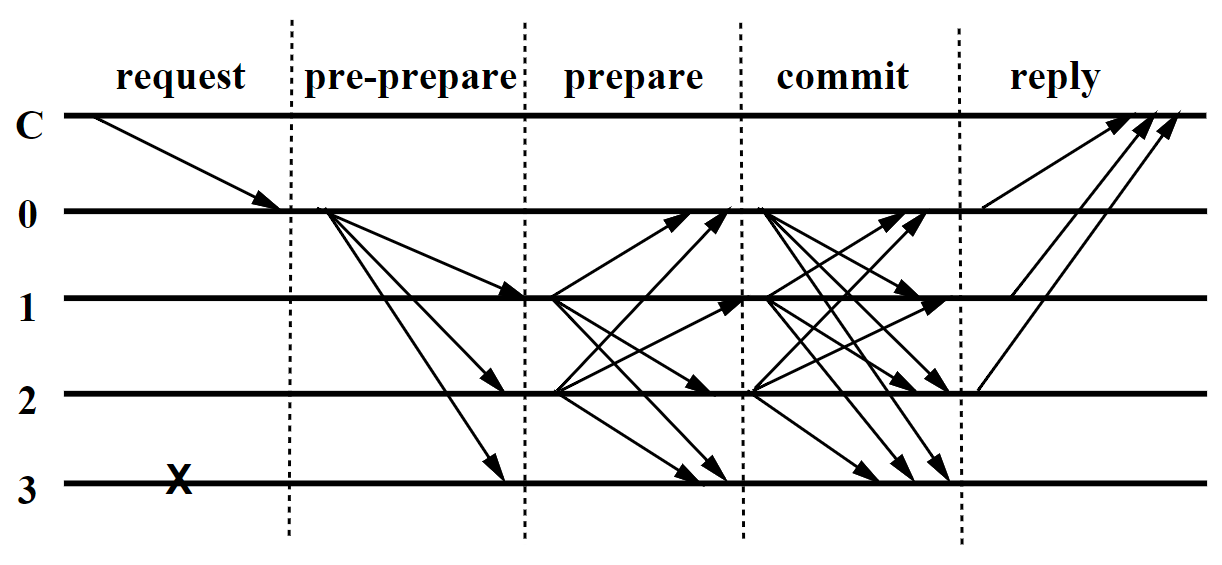
\includegraphics[width=1\textwidth]{pbft.eps}
\caption{정상 케이스 동작(Normal Case Operation)}
\label{fig:1}       %Give a unique label
\end{figure}

\subsection{HotStuff: BFT Consensus with Linearity and Responsiveness}
HotStuff\cite{yin2019hotstuff}은 부분 동기적 모델에서 사용되는 리더 기반 비잔틴 허용 복제 프로토콜이다.
네트워크 통신이 동기적이고 리더가 올바르다면 네트워크 지연속도와 복제본 수에 선형적인 복잡도를 가지고
합의에 도달할 수 있다. HotStuff은 다른 BFT 알고리즘 처럼 \(3f+1\) 개의 노드가 있어야 비잔틴 노드와 관계없이
서비스를 수행할 수 있다. HotStuff은 3단계로 구성된 알고리즘이다. PREPARE, PRE-COMMIT, COMMIT이다.

\textbf{PREPARE 단계.} 새로운 리더가 n-f개의 NEW-VIEW 메시지를 받으면서 단계가 시작된다. 
NEW-VIEW 메시지는 \textit{viewNumber}로 전환될 때 복제본으로 부터 전달되는 메시지이다.
리더는 가장 높은 뷰를 갖는 prepareQC를 선택한다. 이는 \textit{highQC}라 불린다. 리더는 CREATELEAF 메서드와
새로운 제안을 사용하여 \textit{highQC.node}의 꼬리를 확장한다. 메서드는 새로운 리프 노드를 자식으로 두고
내부에 부모의 해시값을 저장하게 한다. 해당 노드를 포함한 PREPARE 메시지를 생성하여 모든 복제본에 전달한다.
수신한 복제본은 SAFENODE를 사용하여 이 메시지를 받아들일지 결정한다. 그리고 제안을 서명한 뒤
PREPARE에 대한 투표를 생성하여 리더에게 보낸다.

\textbf{PRE-COMMIT 단계.} 리더는 \((n-f)\)개의 PREPARE 투표를 받은 뒤 이를 조합하여 \textit{prepareQC}를
형성한다. 리더는 이 \textit{prepareQC}를 PRE-COMMIT 메시지에 담아 브로드캐스트 한다. 수신한 복제본은 리더에게
PRE-COMMIT 투표를 서명과 함께 보낸다.

\textbf{COMMIT 단계.} 커밋 단계는 PRE-COMMIT 단계와 비슷하다. 리더는 \((n-f)\) PRE-COMMIT 투표를 수신한 뒤
(알고리즘1의 2번째 줄)
이를 조합하여 \textit{precommitQC}를 만든다. (알고리즘1의 4번째 줄) 그리고 이를 COMMIT 메시지와 함께 브로드캐스트한다. 
(알고리즘1의 5번째 줄)
이를 수신한 복제본은 COMMIT 메시지에 대한 투표를 보낸다. (알고리즘1의 11번째 줄) 중요한 점은 복제본은 precommitQC에 잠기는 상태가 되는점이다.
따라서 \textit{lockedQC}라는 변수에 \textit{precommitQC} 를 할당한다. (알고리즘1의 9번째 줄) 이것은 제안에 대한 safety속성을 보장하기 위한
매우 중요한 작업이다.

\begin{algorithm}
  \caption{COMMIT 단계}
  \begin{algorithmic}[1]
  \State {as a \textbf{leader}}
    \State \hskip1em wait for \((n-f)\) votes:
      \State \hskip2em $V \leftarrow \{v | MATCHINGMSG(\textit{v}, PRE-COMMIT, \textit{curView})\}$
    \State \hskip1em $\textit{precommitQC} \leftarrow QC(\textit{V})$
    \State \hskip1em broadcast MSG(COMMIT, ⊥, \textit{precommitQC})
  \State {as a \textbf{replica}}
    \State \hskip1em wait for message \textit{m} from LEADER(\textit{curView})
      \State \hskip2em m : MATCHINGQC(\textit{m.justify}, PRE-COMMIT, \textit{curView})
    \State \hskip1em $\textit{lockedQC} \leftarrow QC(\textit{m.justify})$
    \State \hskip1em send to LEADER(\textit{curView})
      \State \hskip2em VOTEMSG(COMMIT, \textit{m.justify.node}, ⊥)
  \end{algorithmic}
\end{algorithm}


\textbf{DECIDE 단계.} 리더는 \((n-f)\)개의 COMMIT 투표를 받은 뒤 이를 조합하여 \textit{commitQC}를
형성한다. 그리고 모든 다른 복제본에 전달한다. 복제본은 \textit{commitQC}를 받자말자 이 쿼럼인증서 안에있는
제안을 확인하고 실행을 한다. 그리고 복제본은 \textit{viewNumber}를 증가시키고 다음 뷰를 시작한다.



\subsection{LibraBFT: BFT Consensus with Linearity and Responsiveness}
LibraBFT는 Libra 블록체인을 위해 비동기 네트워크 환경에서 safety속성을 보장하는 비잔틴 장애 허용 합의 알고리즘이다.
지리적으로 분산된 데이터베이스 간에 상태 머신 복제를 통해 동일한 프로그래밍 가능한 리소스(programmable resources)을
유지할 수 있게한다. 다른 상태 머신 복제 알고리즘과 유사하게 
각 데이터베이스는 순서있는 트랜잭션 목록을 받고 실행하여 동일한 상태를 유지한다.
 이 합의 알고리즘 역시 다른 알고리즘 처럼 \(3f+1\) 개의 노드가 있어야 시스템을 비잔틴 행위로 부터
시스템을 보호할 수 있다. LibraBFT는 HotStuff 알고리즘을 기반으로하는 알고리즘이다. HotStuff 장점으로 다음이 있다.
\begin{itemize}
  \item 합의 결정 비용은 단순히 결정을 각 복제본에 전파하는 것 이상의 비용이 들지 않는다.
  \item 단일 통신 단계를 중심으로 프로토콜이 구축되어 간결하면서도 견고한 블록체인 구현을 할 수 있게 한다.
  \item 공개 모집을 통해 새롭게 모집된 노드를 동적으로 시스템에 추가할 수 있다. 
\end{itemize}

LibraBFT\cite{librabft}는 전통적인 라운드 방식을 적용하며 특히 HotStuff의 3단계 합의 방식을 사용한다.
다른 BFT 알고리즘과 유사하게 각 라운드에는 리더가 지정되고 제안하게 한다. 제안을 받은 각 복제본이 리더가 제안한
내용에 서명을 하고 투표 형태로 다음 라운드의 리더에게 보내게 된다.

LibraBFT는 HotStuff\cite{yin2019hotstuff}의 첫번째, 두번째 단계에서 쿼럼 인증서를 만드는 부분을 차용하고 있다. 각 라운드에서 리더는
쿼럼 인증서를 형성하며 동시에 제안을 형성하여 브로드캐스트하는 것이다. 그리고 이에 대한 투표는 다음 라운드로 넘겨서
무한히 반복하는 방식이다. Figure ~\ref{fig:2}에 보이는 것처럼 실제 커밋은 3-chain commit 라는 규칙을 따른다.

3-chain commit 룰에 대한 설명은 다음과 같다. LibraBFT의 3단계는 각 라운드에 퍼져있다.
예를들어 k라운드에서 리더는 새로운 제안을 한다. k+1 라운드에서는 리더는 다시 새로운 제안을 하며
동시에 k라운드 제안에 대한 투표를 받아서
k라운드 쿼럼 인증서를 형성하고 대한 인증을 진행한다. k+2 라운드 역시 동일하고 k+1라운드의 인증서를 만든다
이때 k부터 k+2라운드까지 쿼럼인증서가 연결된 상태가 되어 커밋될 수 있는 상태가 된다.
Figure ~\ref{fig:2} 와 같이 k+3 라운드가 시작되면서 k라운드에 제안된 명령은 실행되고 커밋된다.
LibraBFT는 이러한 방식을 통해
체인 품질, 낙관적 응답성(optimistic reponsiveness)와 선형성(linearity)을 보장할 수 있다. 

LibraBFT는 리더 기반 알고리즘으로 커밋까지 \(O(n)\) 정도의 메시지 통신 비용이 발생한다. 그리고 비잔틴 노드나
장애로 인해 특정 라운드가 타웃아웃 되더라도 동일하게 \(O(n)\) 의 메시지 통신 비용이 발생한다.

\begin{figure}
  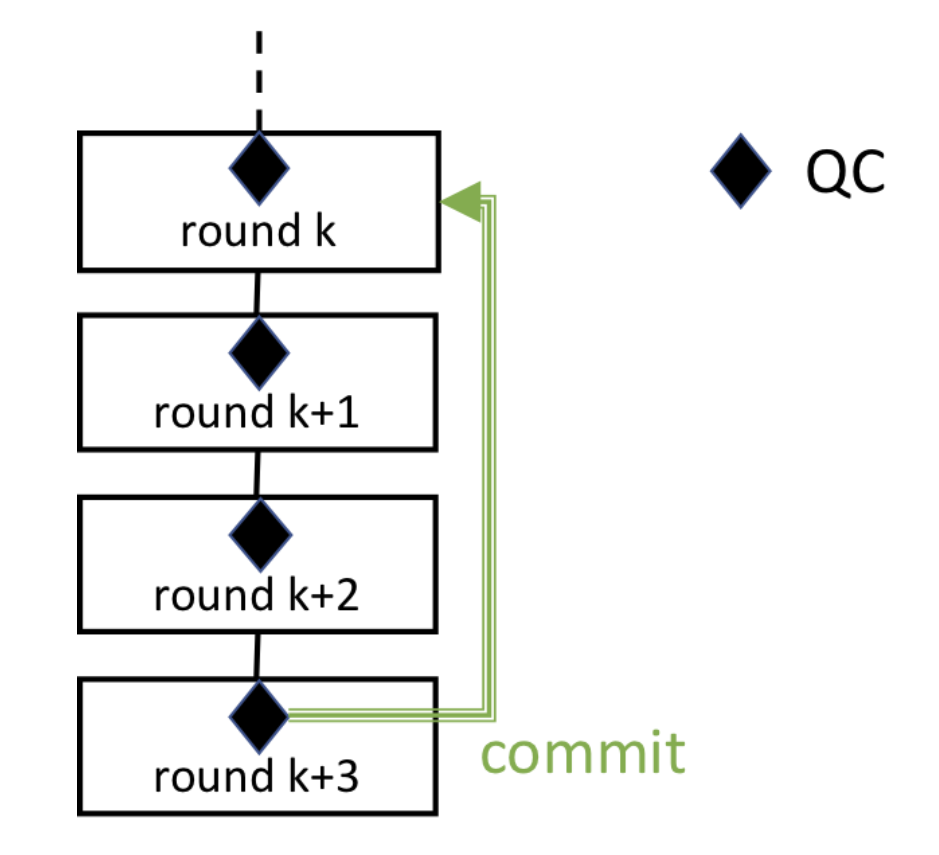
\includegraphics[width=0.5\textwidth]{librabft.eps}
\caption{LibraBFT 단계들은 여러 라운드에 펼쳐져 있음}
\label{fig:2}       %Give a unique label
\end{figure}

\section{토론}
\label{sec:2}

다음은 위에 분석하였던 3개의 알고리즘 성능을 비교할 수 있다. PBFT는 안정적인 리더가 라운드를 진행할때 
커뮤니케이션과 커밋에 2라운드 트립 비용이 \(O(n^{2})\) 이다.
리더를 교체할 경우 모든 복제본들은 VIEW-CHANGE 메시지를 브로드캐스트 한다. 이는 다음 뷰 번호를 알 수 없기때문에
리더에게 직접 보내지 못하기 때문이다. 따라서 메시지를 받은 모든 복제본은 인증서를 검증 하는데 이때 총 \(O(n^{3})\)라는
적지 않은 비용이 발생한다. 

반면 HotStuff는 같은 제안부터 커밋까지 3단계를 갖는 상태 복제 프로토콜이지만, 
리더 중심 프로토콜이기 때문에 주고받는 메시지 숫자가 적다. 리더는 새로운 제안을 모든 복제본에 브로드캐스트하고 
모든 복제본은 그 제안을 받은 뒤 투표를 리더에게만 보낸다. 따라서 복제본이 \textit{N}개라면 \textit{N-1}개의 
제안을 위한 메시지가 발생하고 \textit{N-1}개의 복제본은 투표를 리더에게 직접 보낸다. 이러한 단계가 총 3단계가
존재하며 총 통신 비용은 \(O(n)\)이 된다.

여기에 HotStuff은 이 제안-투표하는 것이 반복되는 것을 최적화 하여 CHAINED-HOTSTUFF를 개발하였다.
같은 \(O(n)\) 이지만 커뮤니케이션 비용이 \(1/3\)로 감소한다. LibraBFT은 이러한 CHAINED-HOTSTUFF를 적용하고 있어서
성능이 우수하다. 차이점이라면 내부적으로 HotStuff과 다른 자료구조를 이용하고 있다는 점이다.

\rowcolors{1}{black!30}{white}
\begin{tcolorbox}[enhanced, notitle, clip upper, title={알고리즘 성능비교}, fontupper=\sffamily,%
    tabularx={>{\cellcolor[gray]{.5}\color{white}}r%
              >{\centering\arraybackslash}X%
              >{\centering\arraybackslash}X}]
  &\cellcolor{black!80}\color{white}올바른 리더 &\cellcolor{black!80}\color{white}결함있는 리더(인증 복잡도) \\
PBFT\cite{castro1999practical} & \(O(n^{2})\) & \(O(n^{3})\) \\
HotStuff\cite{yin2019hotstuff} & \(O(n)\)  & \(O(n)\) \\
LibraBFT\cite{librabft} & \(O(n)\) & \(O(n)\) \\
\end{tcolorbox}

가장 빠른 HotStuff를 사용한다고 가정하고, 앞에 조사한 내용을 바탕으로
현재 주제로 잡고있는 분산 프로그래밍 언어에서 2가지 연구과제를 도출할 수 있다.

\textbf{첫째.} 분산된 노드 간의 원격 메서드 호출의 시퀀스와 HotStuff의 각 라운드를 동기화하지 않고 성능을 
높이면서 안정성을 보장할 수 방법에 대해 연구가 좀더 필요하다. 특정 라운드에서 모든 노드가 동일한 상태에 있으며
각 노드는 결정적인 연산을 수행하는 노드라고 가정해보자.
그리고 다른 노드에 메서드 호출 요청을 하고 응답을 받은 뒤 자신의 상태를 갱신한다. 그리고
이 상태를 모든 노드에 전파해야 하는데 이때 HotStuff 프로토콜을 사용할 수 있다.
하지만 이런 설계를 가져가면 실제 RPC 실행 시간이 지나치게 길어져서 성능에 문제가 있을 수 있다. 그렇다고 모든 노드가
동시에 합의하는 방식으로 가자니 그것 역시 성능에 악영향을 끼치게 된다.

\textbf{둘째.} 상태 복제 알고리즘을 완전히 배제하고 트래픽을 최소화하면서 메시지에 프로그램 실행환경을 
주고 받을 수 있는 방법에 대한 연구도 필요하다. 결국 상태 복제 알고리즘은 3f+1 이라는 조건을 만족했을때
정상적으로 작업을 처리할 수 있기 때문에, 알고리즘을 적용하는 것 자체가 보안적인 결함이 있다고 할 수 있다.

\section{결론}
\label{sec:3}
프로그램 개발에 언어라는 것은 가장 중요한 뼈대이다. 특히 언어에서 런타임이나 VM스펙과 구현체까지 제시해야 하는 
상황에서는 보안을 가장 최우선으로 고려해야 한다. 만약 위 HotStuff 프로토콜을 RPC를 지원하는 분산된 노드에 적용을
한다면, 시스템 운영자에게 3f+1 라는 조건에 대해 설명해야할 수 있으며 다른 여러가지 조건등이 만족되어야 한다. 
이러한 조건들은 다소 기술적인 한계로 보인다. 하지만 컴퓨팅 환경이 과거와 달리 많이 발전하였기 때문에
동기적 모델이나 부분 동기적 모델을 기반으로한 HotStuff 보다 더 실용적인 알고리즘이 등장하는지 지켜보아야 한다.



%Text with citations \cite{RefB} and \cite{RefJ}.

%\begin{acknowledgements}
%If you'd like to thank anyone, place your comments here
%and remove the percent signs.
%\end{acknowledgements}


% Authors must disclose all relationships or interests that 
% could have direct or potential influence or impart bias on 
% the work: 
%
% \section*{Conflict of interest}
%
% The authors declare th at they have no conflict of interest.


% BibTeX users please use one of
%\bibliographystyle{spbasic}      % basic style, author-year citations
%\bibliographystyle{spmpsci}      % mathematics and physical sciences
%\bibliographystyle{spphys}       % APS-like style for physics
\bibliographystyle{unsrt}
\bibliography{references.bib}
% name your BibTeX data base asd

% Non-BibTeX users please use  
  %\begin{thebibliography}{asdf}
%
% and use \bibitem to create references. Consult the Instructions
% for authors for reference list style.
%
  %\bibitem{RefJ}
% Format for Journal Reference
  %Author, Article title, Journal, Volume, page numbers (year)
% Format for books
  %\bibitem{RefB}
  %Author, Book title, page numbers. Publisher, place (year)
% etc
  %\end{thebibliography}
        % qhe.bib is the name of our database
     
\end{document}
% end of file template.tex

